\usetikzlibrary{calc}
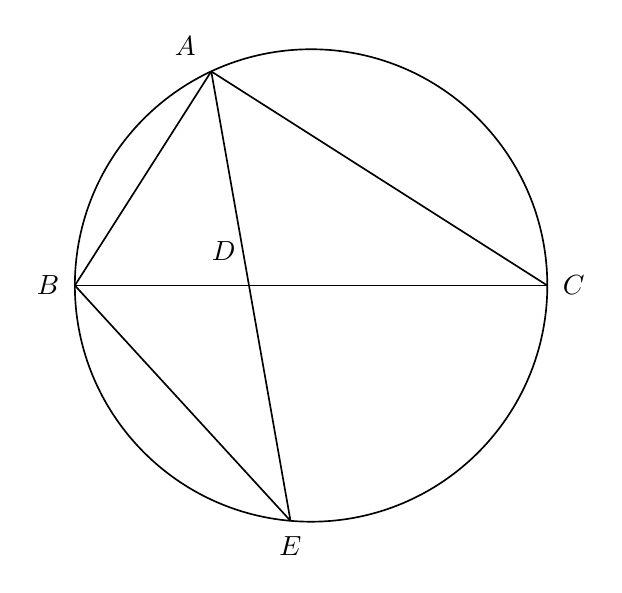
\begin{tikzpicture}[x=1cm,y=1cm,line width=.6pt,font=\normalsize]
\coordinate (O) at (0,0);
\coordinate (A) at (-1.2679,2.7189);
\coordinate (B) at (-3,0);
\coordinate (C) at (3,0);
\coordinate (E) at (-0.2615,-2.9886);
\coordinate (D) at (-0.7884,0);
\draw (O) circle[radius=3cm];
\draw (A)--(B);
\draw (A)--(C);
\draw (A)--(E);
\draw (B)--(C);
\draw (B)--(E);
\node[above left=2pt] at (A) {$A$};
\node[left=2pt] at (B) {$B$};
\node[right=2pt] at (C) {$C$};
\node[below=2pt] at (E) {$E$};
\node at ($(D)+(-0.32,0.44)$) {$D$};
\end{tikzpicture}
